\documentclass[ignorenonframetext,]{beamer}
\setbeamertemplate{caption}[numbered]
\setbeamertemplate{caption label separator}{: }
\setbeamercolor{caption name}{fg=normal text.fg}
\beamertemplatenavigationsymbolsempty
\usepackage{lmodern}
\usepackage{amssymb,amsmath}
\usepackage{ifxetex,ifluatex}
\usepackage{fixltx2e} % provides \textsubscript
\ifnum 0\ifxetex 1\fi\ifluatex 1\fi=0 % if pdftex
  \usepackage[T1]{fontenc}
  \usepackage[utf8]{inputenc}
\else % if luatex or xelatex
  \ifxetex
    \usepackage{mathspec}
  \else
    \usepackage{fontspec}
  \fi
  \defaultfontfeatures{Ligatures=TeX,Scale=MatchLowercase}
\fi
\usetheme[]{CambridgeUS}
\usecolortheme{beaver}
\usefonttheme{structurebold}
% use upquote if available, for straight quotes in verbatim environments
\IfFileExists{upquote.sty}{\usepackage{upquote}}{}
% use microtype if available
\IfFileExists{microtype.sty}{%
\usepackage{microtype}
\UseMicrotypeSet[protrusion]{basicmath} % disable protrusion for tt fonts
}{}
\newif\ifbibliography
\hypersetup{
            pdftitle={A3 The GESIS Panel data},
            pdfauthor={Jan-Philipp Kolb},
            pdfborder={0 0 0},
            breaklinks=true}
\urlstyle{same}  % don't use monospace font for urls
\usepackage{graphicx,grffile}
\makeatletter
\def\maxwidth{\ifdim\Gin@nat@width>\linewidth\linewidth\else\Gin@nat@width\fi}
\def\maxheight{\ifdim\Gin@nat@height>\textheight0.8\textheight\else\Gin@nat@height\fi}
\makeatother
% Scale images if necessary, so that they will not overflow the page
% margins by default, and it is still possible to overwrite the defaults
% using explicit options in \includegraphics[width, height, ...]{}
\setkeys{Gin}{width=\maxwidth,height=\maxheight,keepaspectratio}

% Prevent slide breaks in the middle of a paragraph:
\widowpenalties 1 10000
\raggedbottom

\AtBeginPart{
  \let\insertpartnumber\relax
  \let\partname\relax
  \frame{\partpage}
}
\AtBeginSection{
  \ifbibliography
  \else
    \let\insertsectionnumber\relax
    \let\sectionname\relax
    \frame{\sectionpage}
  \fi
}
\AtBeginSubsection{
  \let\insertsubsectionnumber\relax
  \let\subsectionname\relax
  \frame{\subsectionpage}
}

\setlength{\parindent}{0pt}
\setlength{\parskip}{6pt plus 2pt minus 1pt}
\setlength{\emergencystretch}{3em}  % prevent overfull lines
\providecommand{\tightlist}{%
  \setlength{\itemsep}{0pt}\setlength{\parskip}{0pt}}
\setcounter{secnumdepth}{0}

\title{A3 The GESIS Panel data}
\author{Jan-Philipp Kolb}
\date{06 August 2018}

\begin{document}
\frame{\titlepage}

\begin{frame}{Das GESIS Panel}

\begin{itemize}
\tightlist
\item
  Wahrscheinlichkeitsbasiertes Access Panel für Individuen: - Allgemeine
  Bevölkerung in Deutschland, Deutschsprachhige Bevölkerung, 18-70 Jahre
\item
  Panelisten wurden aus den Melderegistern rekrutiert - (270 Sampling
  Points) 7599 face-to-face Interviews (CAPI)
\item
  Ungefähr 5000 Panelisten (Basis Stichprobe / erste Kohorte 2014)
\end{itemize}

\end{frame}

\begin{frame}{Das GESIS Panel Campus File}


\includegraphics{figure/gpdata.PNG}

\end{frame}

\begin{frame}[fragile]{Download data}

\begin{itemize}
\tightlist
\item
  Übersichtsseite:
  \href{https://www.gesis.org/gesis-panel/data/gesis-panel-campus-file/}{\textbf{GESIS
  Panel Campus File}}
\item
  Registrierung notwendig
\end{itemize}

\begin{block}{Links für den Download:}

\begin{itemize}
\tightlist
\item
  \href{https://dbk.gesis.org/dbksearch/download.asp?db=D\&id=62367}{\textbf{Download
  \texttt{.csv}}}
\item
  \href{https://dbk.gesis.org/dbksearch/download.asp?db=D\&id=62369}{\textbf{Download
  \texttt{.sav}}}
\item
  \href{https://dbk.gesis.org/dbksearch/download.asp?db=D\&id=62371}{\textbf{Download
  \texttt{**14.dta}}}
\end{itemize}

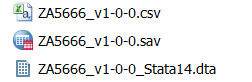
\includegraphics{figure/filenamesGP2.PNG}

\end{block}

\end{frame}

\begin{frame}{Einen ersten Eindruck von den Daten bekommen}

\begin{itemize}
\tightlist
\item
  bbzc022a - Häufigkeit politische Nachrichten
\item
  bfam051a - MPMB Capacity: Termine fallen rechtzeitig ein
\item
  bfzi023a - Umfragen GESIS GM: Interessant
\item
  baai124a - Schwierigkeit Fragebogen zu verstehen
\end{itemize}

\begin{tabular}{l|l|l|l}
\hline
bbzc022a & bfam051a & bfzi023a & baai124a\\
\hline
Täglich weniger als eine Stunde & Eher selten & 7 Stimme voll und ganz zu & Etwas schwierig\\
\hline
Täglich weniger als eine Stunde & Eher oft & 6 & Überhaupt nicht schwierig\\
\hline
Täglich weniger als eine Stunde & Eher selten & 2 & Etwas schwierig\\
\hline
Einmal im Monat oder seltener & Eher oft & 7 Stimme voll und ganz zu & Überhaupt nicht schwierig\\
\hline
Täglich weniger als eine Stunde & Eher oft & 3 & Überhaupt nicht schwierig\\
\hline
Einmal in der Woche & Not reached & 4 & Etwas schwierig\\
\hline
\end{tabular}

\end{frame}

\begin{frame}[fragile]{Die Variablennamen im GESIS Panel}

\begin{block}{Beispiel für die Zusammensetzung der Variablennamen}

\begin{verbatim}
## [1] "bezf044a" "bdze018a" "bdao036b" "bfzi029a" "bezg091a"
\end{verbatim}

\begin{itemize}
\tightlist
\item
  Die ersten beiden Buchstaben enthalten die Welle:
\end{itemize}

\begin{tabular}{r|l|l}
\hline
year & waves & numbers\\
\hline
2013 & aa,ab,ac,ad,ae,af & 1-6\\
\hline
2014 & ba,bb,bc,bd,be,bf & 7-12\\
\hline
2015 & ca,cb,cc,cd,ce,cf & 13-18\\
\hline
2016 & da,db,dc,dd,de,df & 19-24\\
\hline
2017 & ea,eb,ec,ed,ee,ef & 25-30\\
\hline
2018 & fa,fb,fc,fd,fe,ff & 31-36\\
\hline
\end{tabular}

\begin{itemize}
\tightlist
\item
  Bis zum jetzigen Zeitpunkt sind 34 gelaufen
\end{itemize}

\end{block}

\end{frame}

\begin{frame}{Die Variablennamen im GESIS Panel II}

\begin{itemize}
\tightlist
\item
  Die Stellen drei und vier geben Information über die Studie:
\end{itemize}

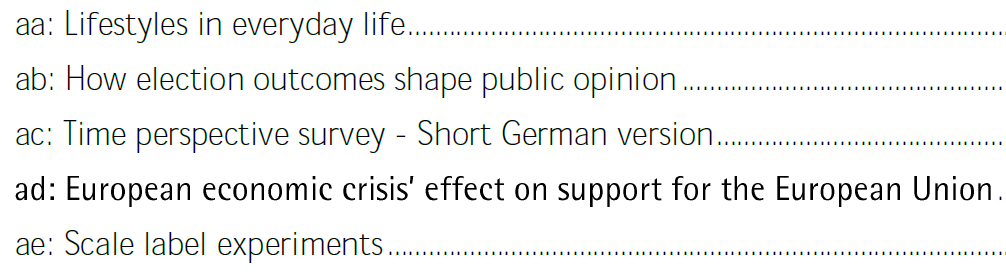
\includegraphics{figure/examplestudies.PNG}

\begin{itemize}
\item
  Die Stellen fünf, sechs und sieben indizieren die Variablennummer
\item
  Die letzte Stelle enthält die Information, ob es sich um eine
  originale Variable (a) oder eine synthetische Variable handelt
  (b,c,d,e,\ldots{})
\end{itemize}

\end{frame}

\begin{frame}[fragile]{Variablennamen im GESIS Panel}

\begin{block}{Beispiel Geburtsdatum - \texttt{cfzh072c}}

\begin{verbatim}
## [1] "cfzh072c"
\end{verbatim}

\begin{verbatim}
## [1] "Welle:  cf"
\end{verbatim}

\begin{verbatim}
## [1] "Studie:  zh"
\end{verbatim}

\begin{verbatim}
## [1] "Variablen Nr.:  072"
\end{verbatim}

\begin{verbatim}
## [1] "Synthetische Variable?:  c"
\end{verbatim}

\end{block}

\end{frame}

\begin{frame}{Die Variablen im Campus File}

\url{https://rpubs.com/Japhilko82/VarsGesisPanel}

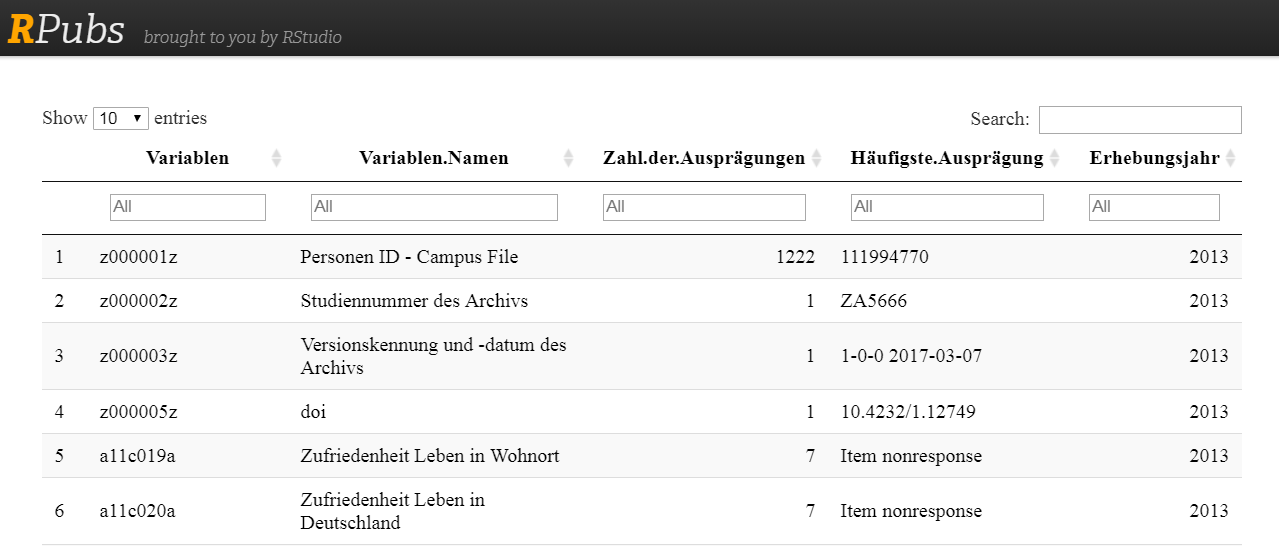
\includegraphics{figure/rpubs_varspuf.PNG}

\end{frame}

\begin{frame}[fragile]{Wellen im Campus File}

\begin{itemize}
\tightlist
\item
  Welche Wellen sind im Campus file?
\item
  Anzahl Variablen pro Welle im Campus File:
\end{itemize}

\begin{verbatim}
## waves
##  a1  ba  bb  bc  bd  be  bf  z0 
## 171 171 154 155 224 185 128   4
\end{verbatim}

\end{frame}

\begin{frame}{Studien im Campus File}

\begin{tabular}{l|l|l}
\hline
  & Name & Code\\
\hline
9 & GESIS Panel Core Study Module - Subjective Well-being & zb\\
\hline
10 & Environmental Spatial Strategies & ag\\
\hline
11 & Cross-National Replication of Question Design Experiments & ah\\
\hline
12 & Survey Evaluation Items & ai\\
\hline
13 & GESIS Panel Core Study Module - Survey Administration Variables & za\\
\hline
14 & GESIS Panel Core Study Module - Monitoring quality: survey experience \& mode characteristics & zq\\
\hline
15 & GESIS Panel Core Study Module - Social and Political Participation & zc\\
\hline
16 & Critical Elections in the European Union & aj\\
\hline
17 & International panel comparison study & ak\\
\hline
18 & Standardization of the Positive and Negative Affect Schedule (PANAS) & al\\
\hline
19 & GESIS Panel Core Study Module - Environmental attitudes and behavior & zd\\
\hline
20 & Short version of the Metacognitive Prospective Memory Battery (MPMBs) & am\\
\hline
21 & Leisure travel and subjective well-being & an\\
\hline
22 & GESIS Panel Core Study Module - Personality and Personal Values & ze\\
\hline
23 & Social and individual predictors of Doing Beauty & ao\\
\hline
24 & Citizens Conception of Democracy and their Political Participation & ap\\
\hline
25 & GESIS Panel Core Study Module - Media Usage & zf\\
\hline
26 & GESIS Panel Longitudinal Core Study Module - Annual Update of Socio-Demography & zh\\
\hline
27 & GESIS Panel Core Study Module - Work and Leisure & zg\\
\hline
28 & Pro-environmental Behavior in High Cost Situations & aq\\
\hline
29 & GESIS Panel Core Study Module - Panel survey participation evaluation \& mode preferences & zi\\
\hline
30 & Policy preferences for inheritance taxes and motives of intergenerational transfers & ar\\
\hline
\end{tabular}

\end{frame}

\begin{frame}{Die Missing Codes im GESIS Panel}

\begin{table}[H]
\centering\begingroup\fontsize{7}{9}\selectfont

\begin{tabular}{r|l|l}
\hline
Value & Value.label & Remark\\
\hline
-11 & Not invited & only in recruitment waves - when profile survey not finished\\
\hline
-22 & Not in panel & not willing to join the panel after recruitment or signing off\\
\hline
-33 & Unit nonresponse & invited but not participating in corresponding wave\\
\hline
-44 & Missing by m.o.p. & mode of participation (m.o.p.): online or offline\\
\hline
-55 & Missing by technical error & e.g. questionnaire programming error\\
\hline
-66 & Missing by design & experimental variation\\
\hline
-77 & Not reached & only in online mode: panelist has not seen the item\\
\hline
-88 & Missing by filter & filtered item\\
\hline
-99 & Item nonresponse & due to nonresponse by the respondent\\
\hline
-111 & Ambiguous answer & ambiguous answers in questionnaire\\
\hline
\end{tabular}\endgroup{}
\end{table}

\end{frame}

\begin{frame}{Zufriedenheit Leben in Wohnort (a11c019a)}

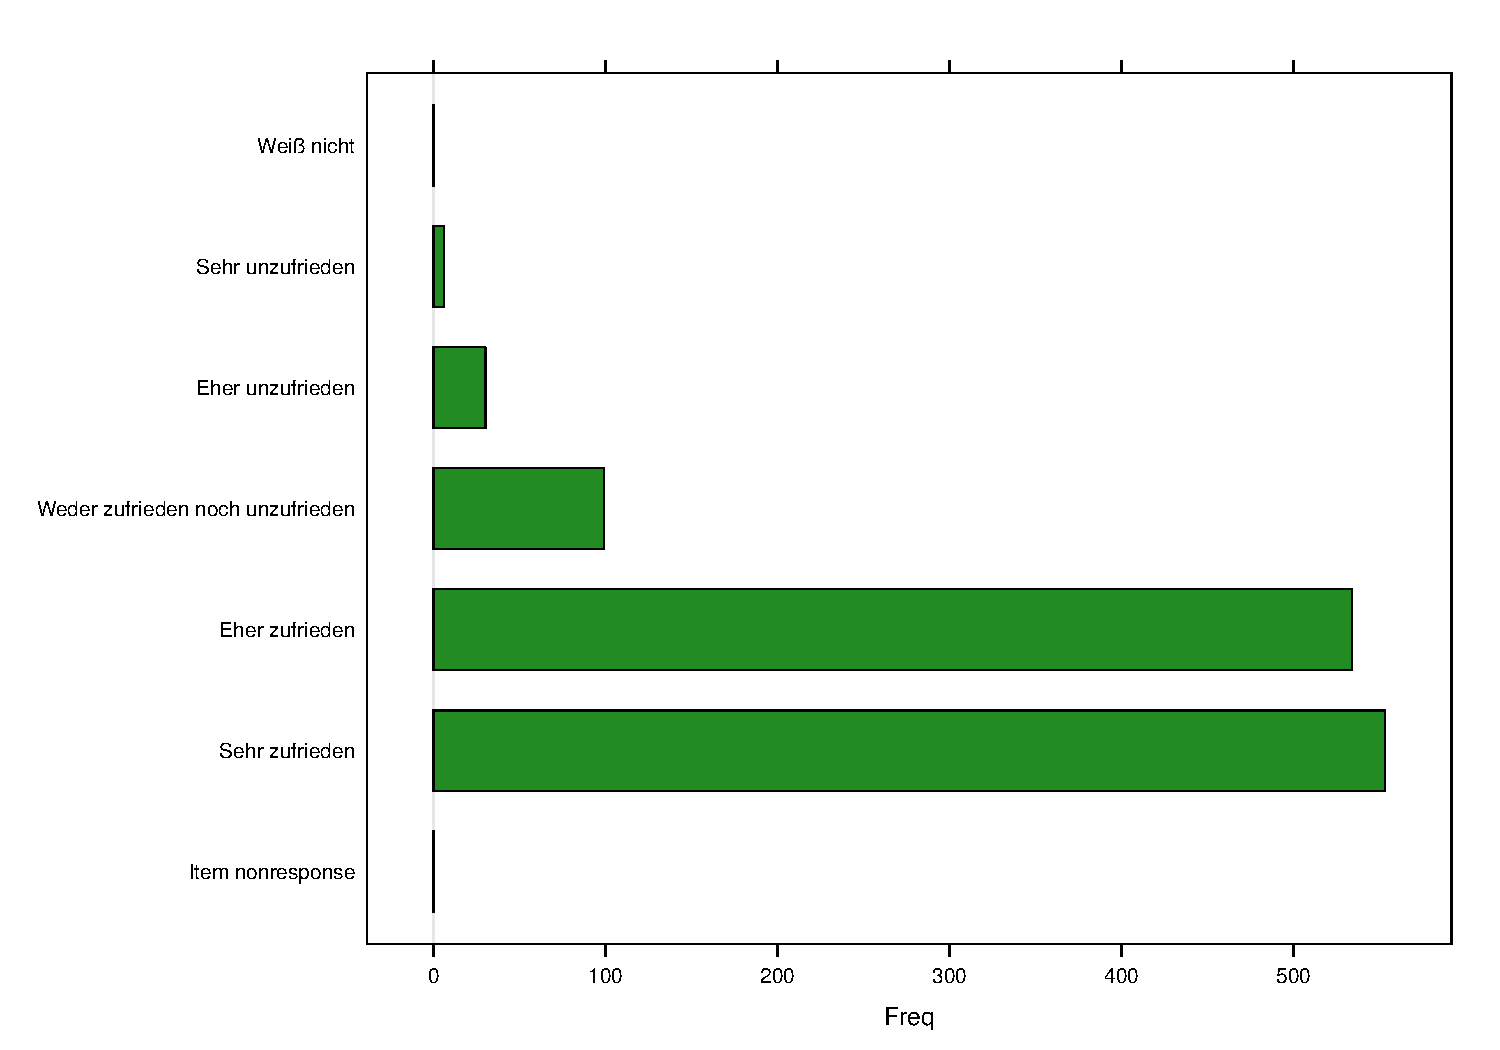
\includegraphics{A3_GESISPanel_files/figure-beamer/unnamed-chunk-25-1.pdf}

\end{frame}

\begin{frame}{Das Codebuch}

\begin{itemize}
\tightlist
\item
  Das Codebuch kann man
  \href{https://www.gesis.org/gesis-panel/documentation/}{\textbf{hier}}
  bekommen.
\end{itemize}

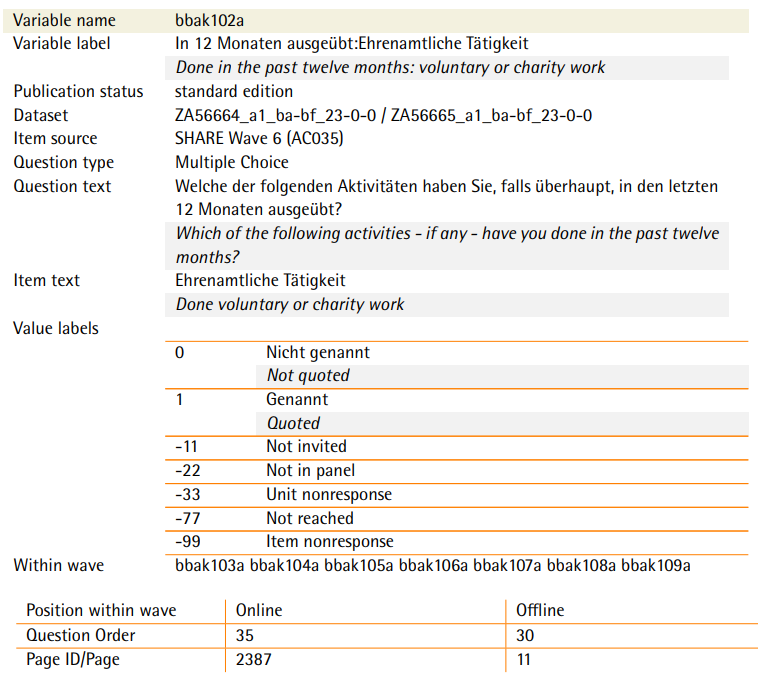
\includegraphics{figure/cdb_bbak102a.PNG}

\end{frame}

\begin{frame}[fragile]{A3A Aufgabe - Download der GESIS Panel Daten}

\begin{itemize}
\tightlist
\item
  Die \texttt{**14.dta} Datei des GESIS Panel Campus file herunterladen.
\end{itemize}

\end{frame}

\end{document}
